\section{Regressão nas Unidades dos Dados, Diagnósticos e Qualidade}

\begin{frame}{A Reta nas Unidades Originais}
    \begin{itemize}
        \item Desfazendo a Z-normalização, chegamos à equação clássica da reta:
        $$\hat{y} = \beta X + \alpha$$
        \item \textbf{Fórmula do Coeficiente Angular (Slope $\beta$):}
        $$\beta = r \cdot \frac{s_y}{s_x}$$
        \item \textbf{Fórmula do Coeficiente Linear (Intercepto $\alpha$):}
        $$\alpha = \bar{Y} - \beta \bar{X}$$
        \item \textbf{Interpretação Prática:}
        \begin{itemize}
            \item \textbf{Slope} ($\beta$): Para cada acréscimo de uma unidade física em $X$, a predição $\hat{Y}$ aumenta em $\beta$ unidades físicas de $Y$.
            \item \textbf{Intercepto} ($\alpha$): Representa a predição para $Y$ caso a variável preditora $X$ assuma o valor zero (deve-se tomar cuidado com a extrapolação fora do domínio amostral).
        \end{itemize}
    \end{itemize}
\end{frame}

\begin{frame}{Qualidade do Ajuste: Coeficiente de Determinação}
    \begin{itemize}
        \item O \textbf{Coeficiente de Determinação} ($R^2$) indica a proporção da variabilidade da variável resposta $Y$ que é explicada pelo modelo linear:
        $$R^2 = 1 - \frac{\sum_{i=1}^N (y_i - \hat{y}_i)^2}{\sum_{i=1}^N (y_i - \bar{Y})^2}$$
        \item \textbf{Propriedades de $R^2$:}
        \begin{itemize}
            \item Na regressão linear simples, vale exatamente o quadrado do coeficiente de Pearson ($R^2 = r^2$).
            \item Varia no intervalo $[0, 1]$ para regressões de mínimos quadrados comuns.
            \item Exemplo: $R^2 = 0.65 \implies 65\%$ da variação dos dados de Y é capturada pelo comportamento linear em relação a X.
        \end{itemize}
    \end{itemize}
\end{frame}

\begin{frame}{Diagnósticos Visuais de Regressão}
    \begin{itemize}
        \item O \textbf{Gráfico de Resíduos} (Residual Plot) é a principal ferramenta de diagnóstico visual. Consiste em plotar os resíduos $e_i = y_i - \hat{y}_i$ contra o preditor $x_i$.
        \item \textbf{Suposição de Homocedasticidade:} A variabilidade dos resíduos deve ser constante ao longo de todo o eixo X.
        \item \textbf{Padrões Indesejados a Detectar:}
        \begin{enumerate}
            \item \textbf{Não-Linearidade:} Resíduos formam curvas (ex: padrão em U). Sugere necessidade de transformações ou modelos não-lineares.
            \item \textbf{Heterocedasticidade:} Resíduos apresentam-se em forma de funil (dispersão aumenta com X). Afeta a validade das inferências e testes de hipóteses clássicos.
        \end{enumerate}
    \end{itemize}
\end{frame}

\begin{frame}{Diagnósticos Visuais: Exemplos Gráficos}
    \begin{columns}[onlytextwidth]
        \begin{column}{0.32\textwidth}
            \centering
            \textbf{\small{1. Homocedástico}} \\
            \vspace{0.1cm}
            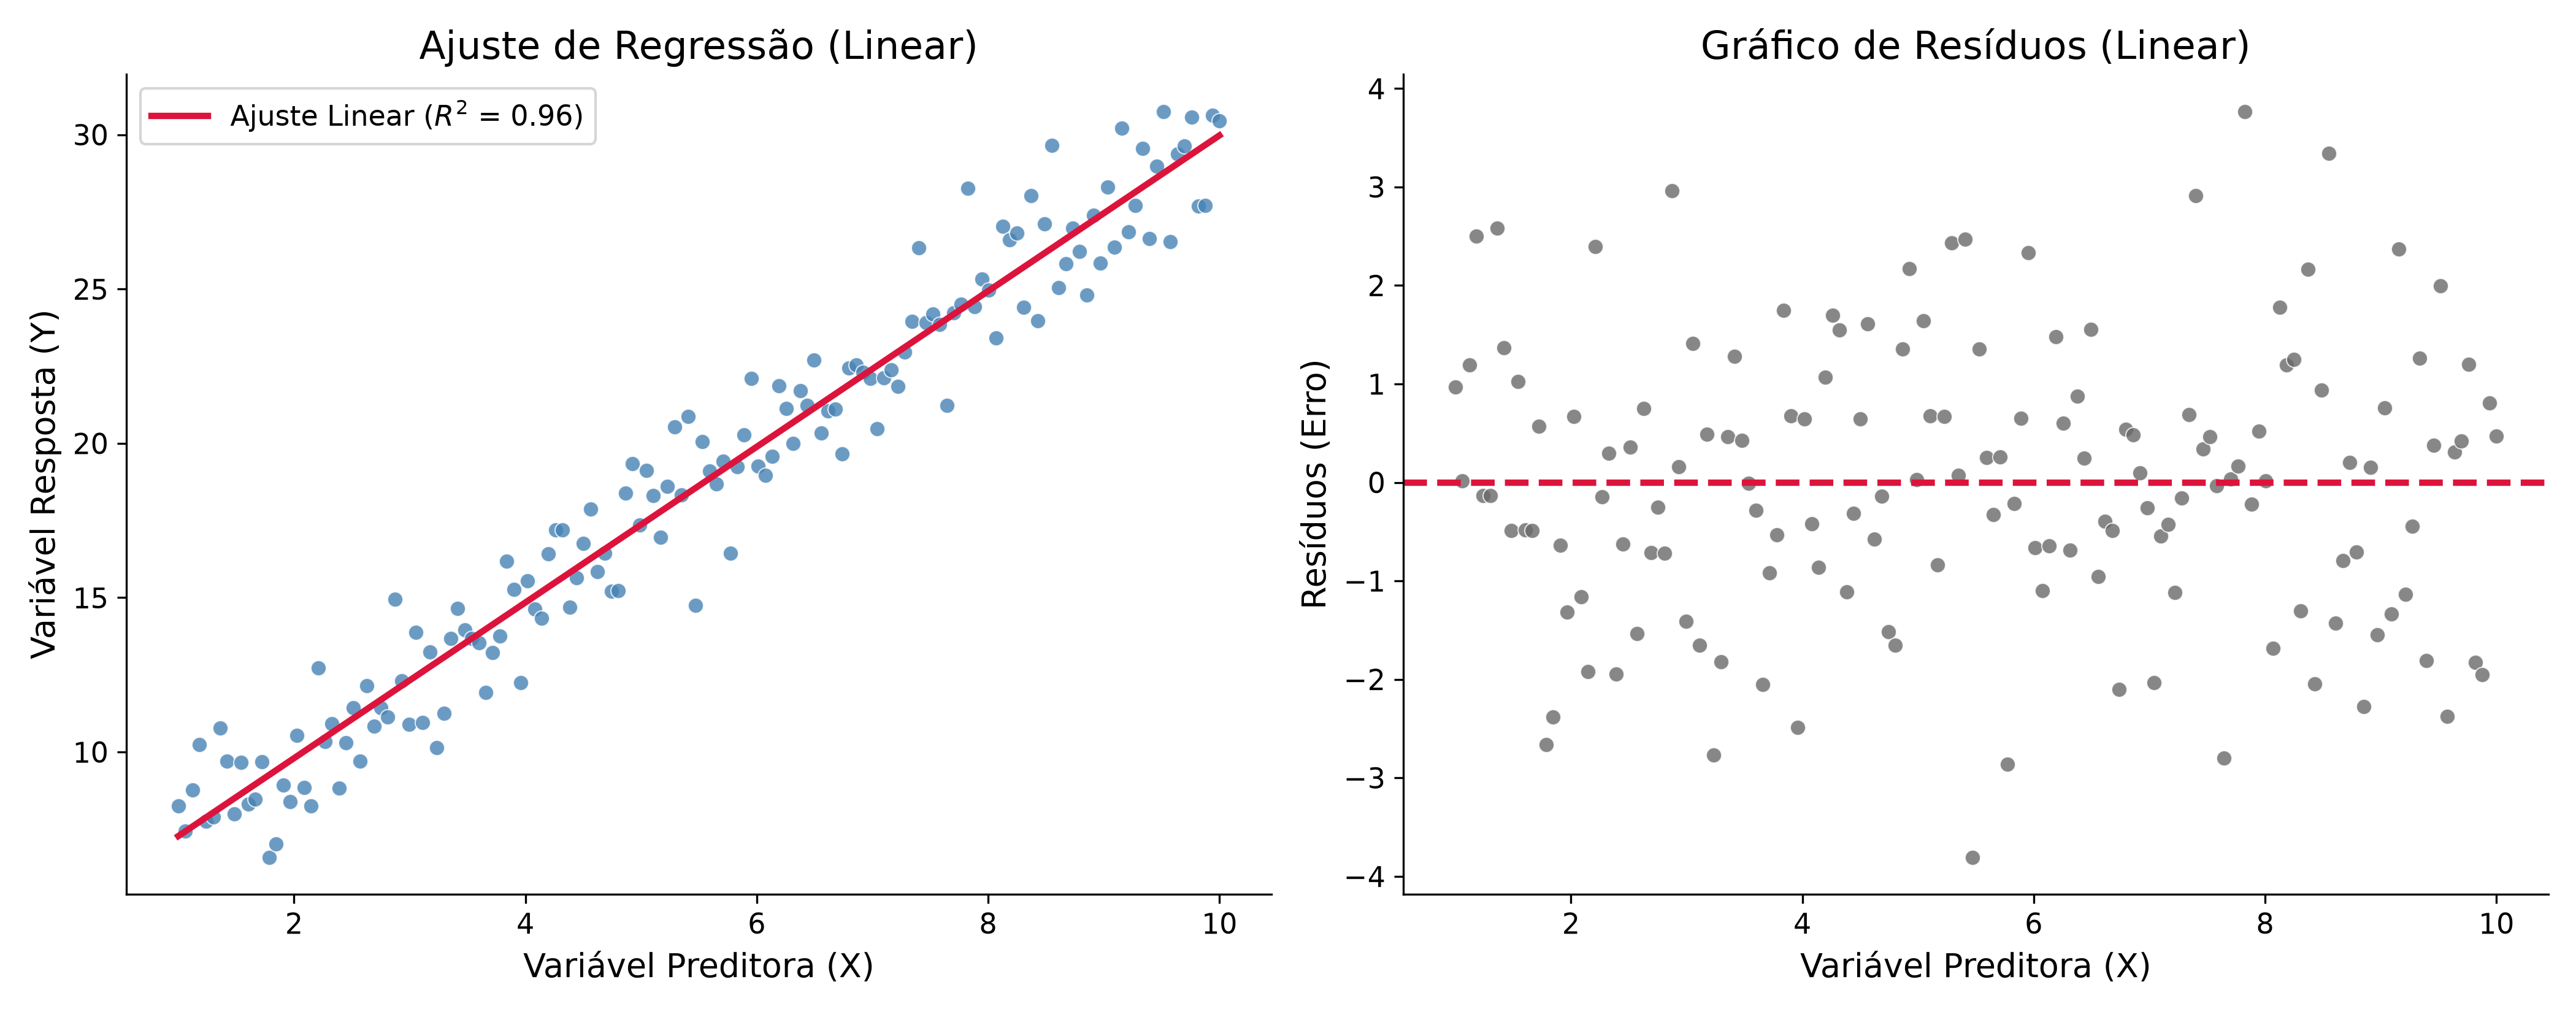
\includegraphics[width=\textwidth]{diagnostico_linear.png} \\
            \vspace{0.1cm}
            \scriptsize{Ideal: dispersão dos resíduos é constante.}
        \end{column}
        \begin{column}{0.32\textwidth}
            \centering
            \textbf{\small{2. Não-Linear}} \\
            \vspace{0.1cm}
            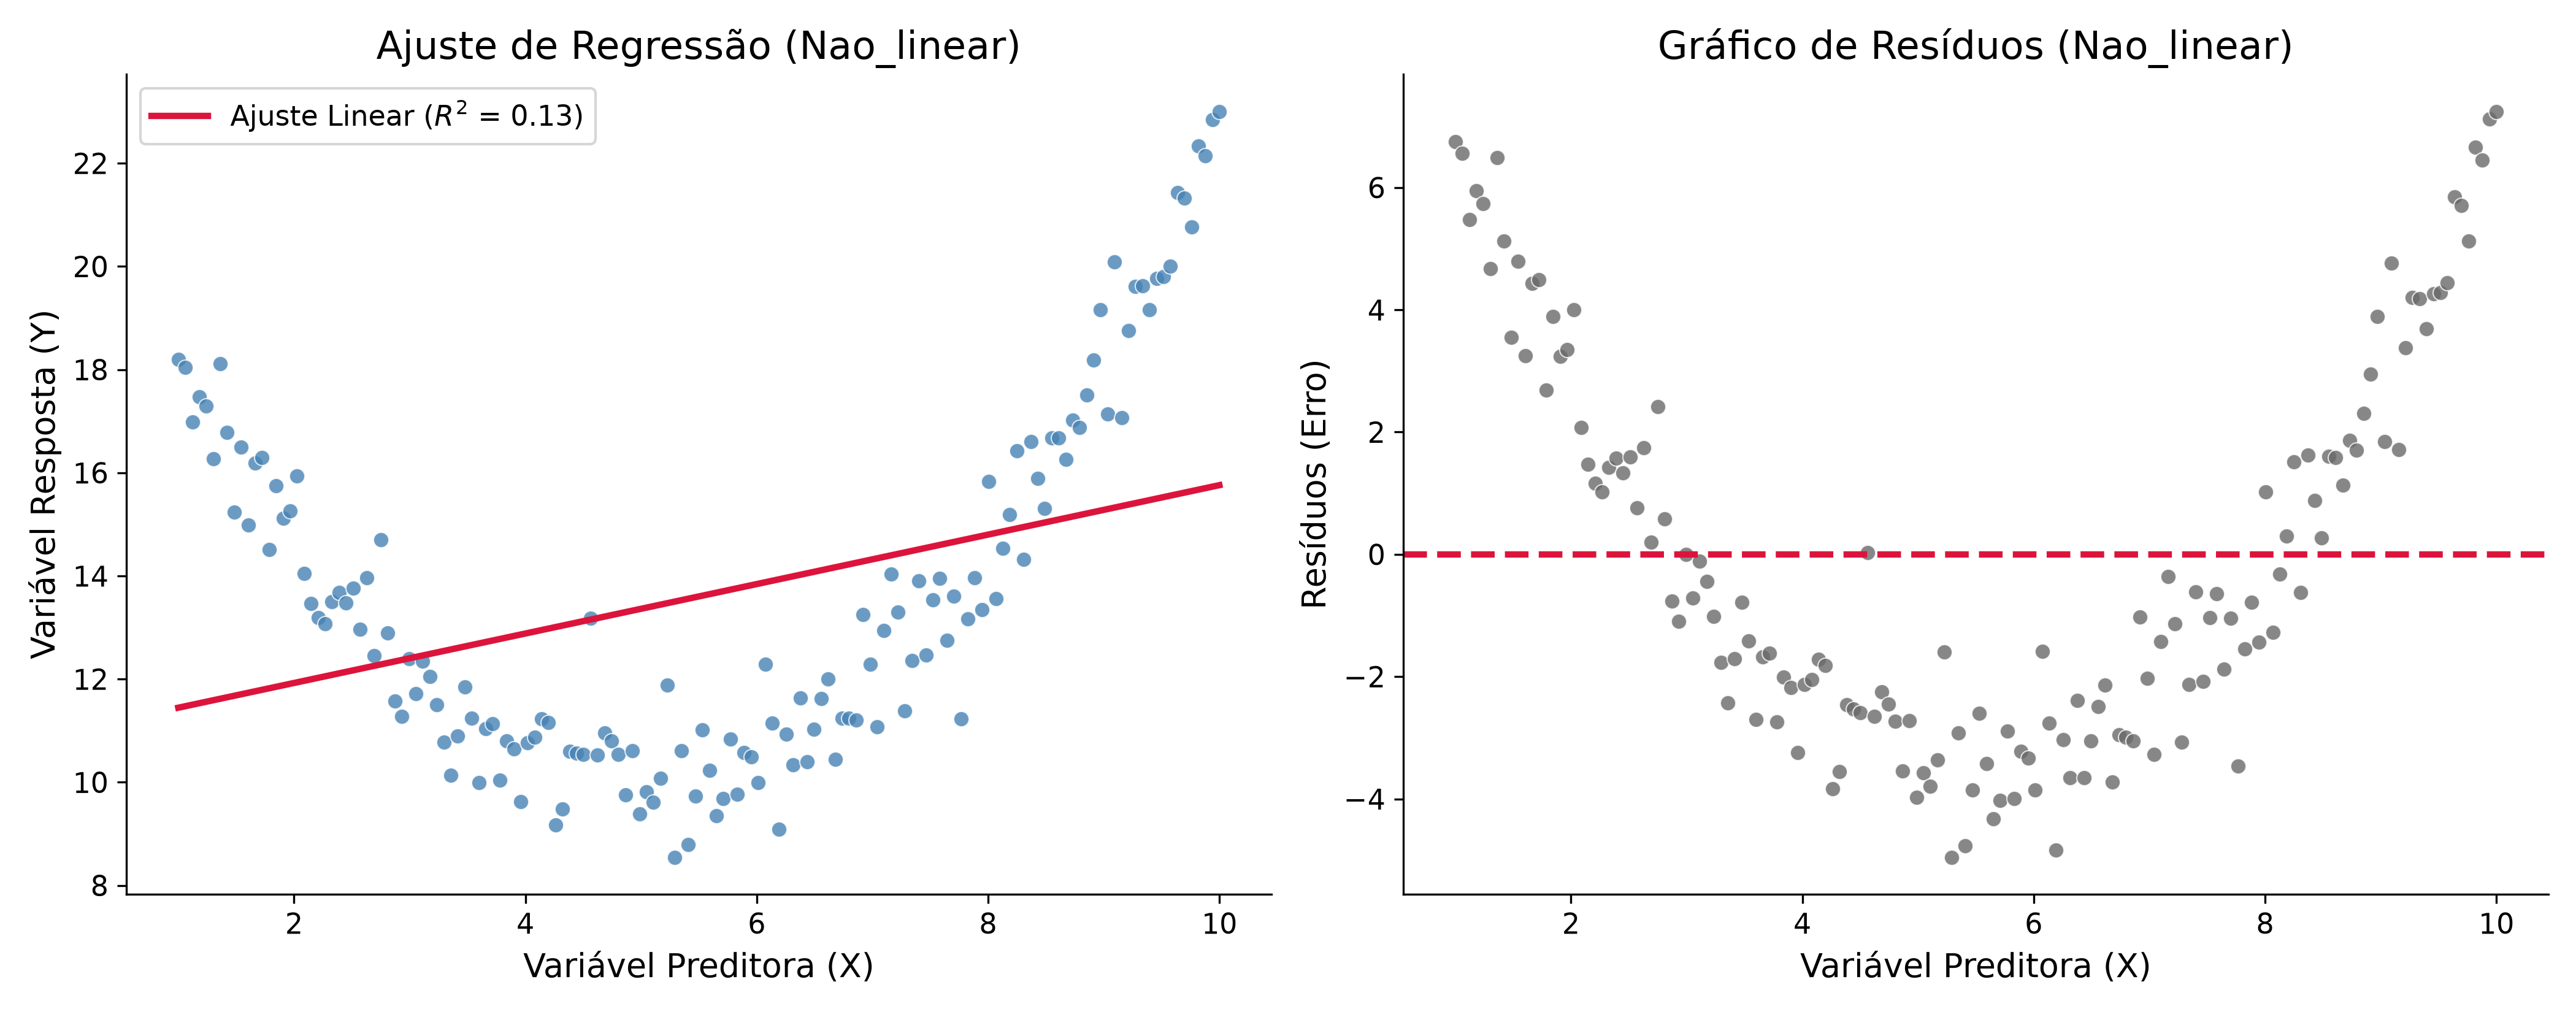
\includegraphics[width=\textwidth]{diagnostico_nao_linear.png} \\
            \vspace{0.1cm}
            \scriptsize{Curvatura: relação não segue padrão linear.}
        \end{column}
        \begin{column}{0.32\textwidth}
            \centering
            \textbf{\small{3. Heterocedástico}} \\
            \vspace{0.1cm}
            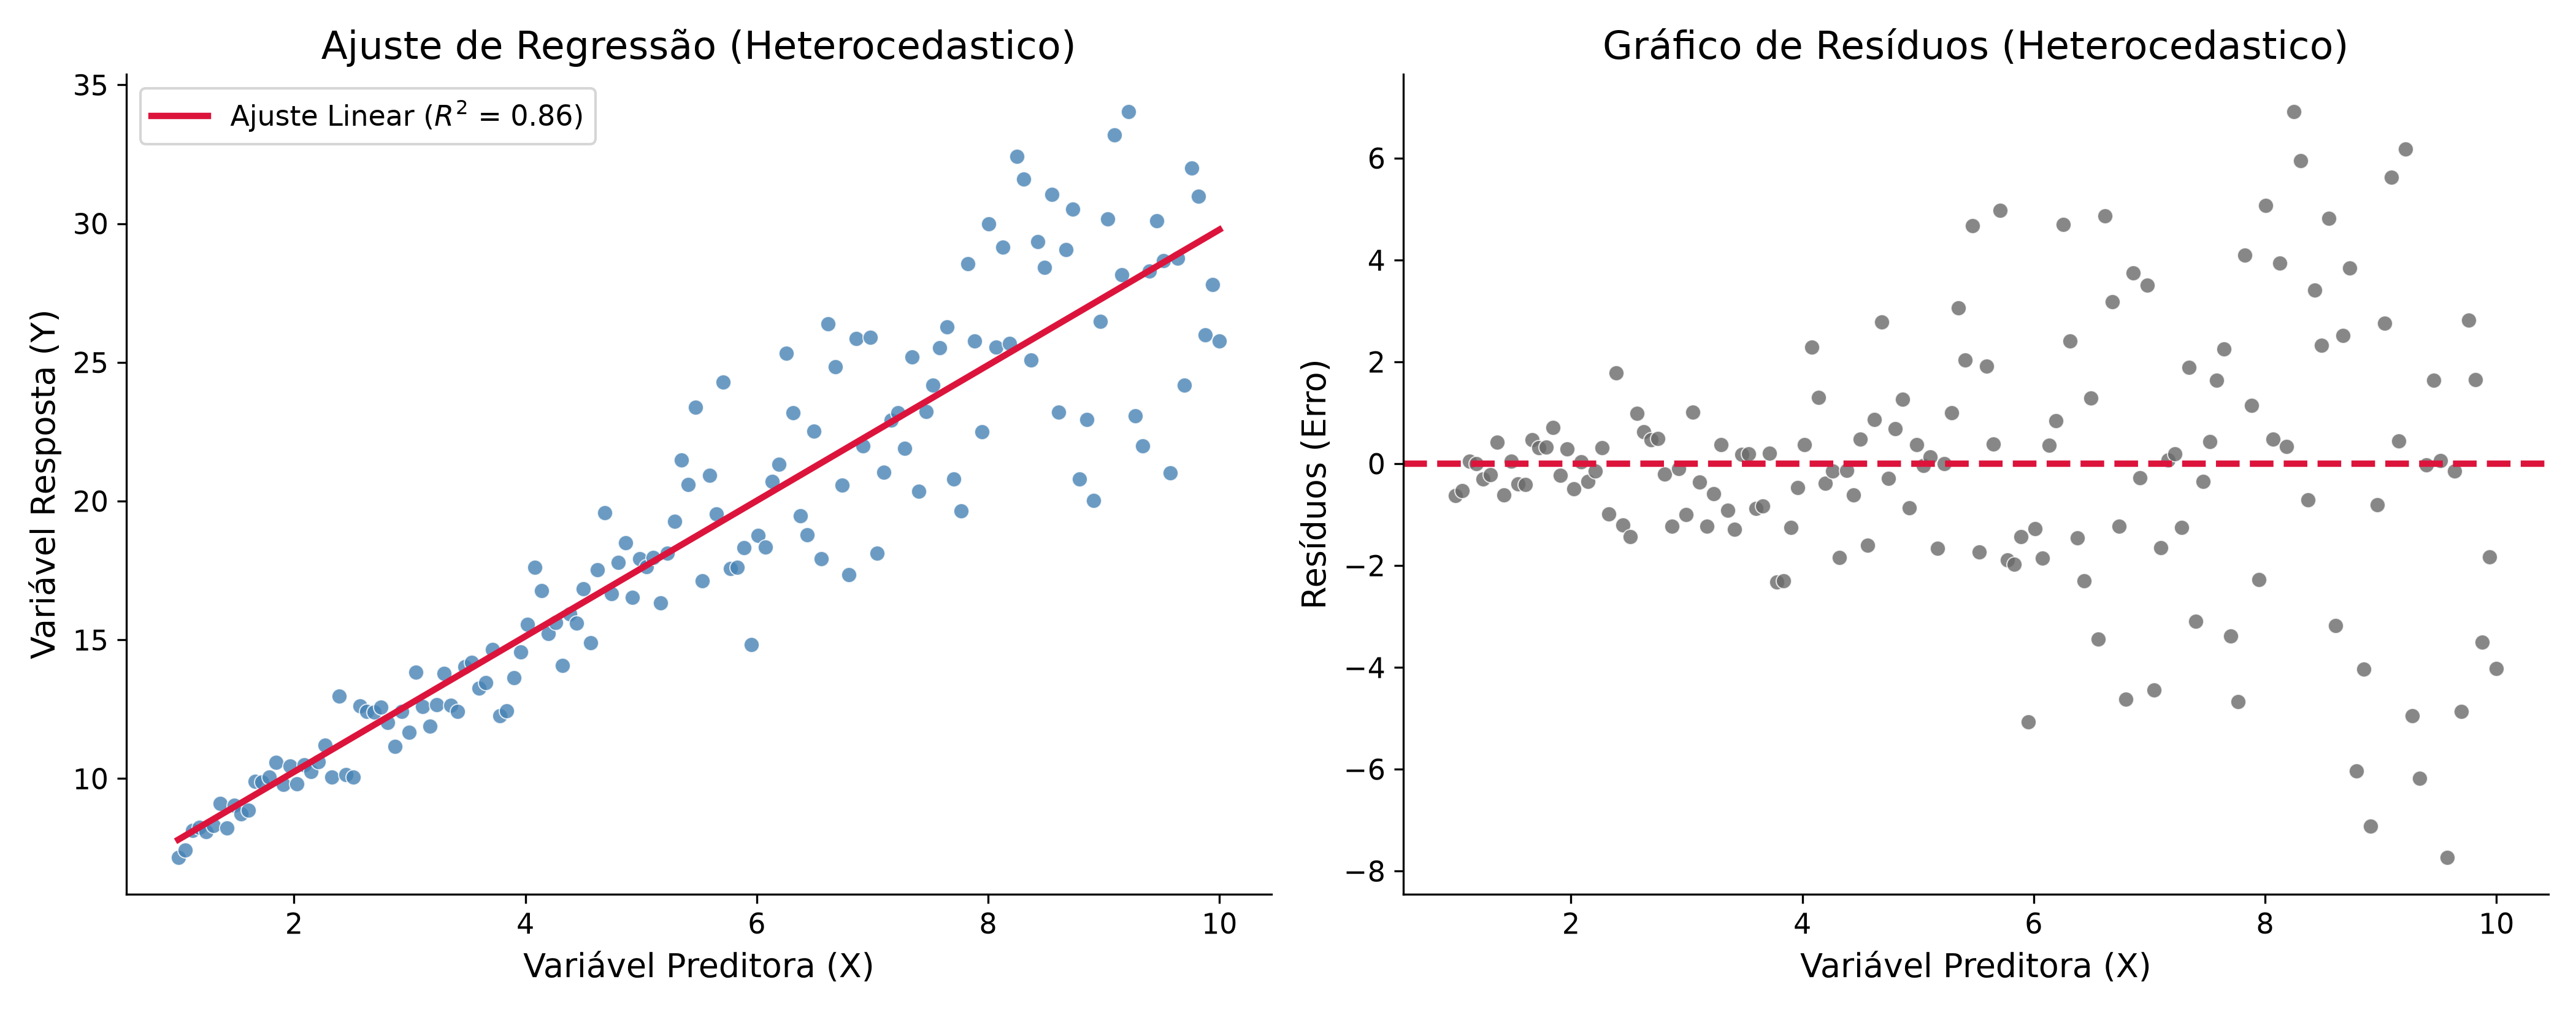
\includegraphics[width=\textwidth]{diagnostico_heterocedastico.png} \\
            \vspace{0.1cm}
            \scriptsize{Funil: variância aumenta com a variável X.}
        \end{column}
    \end{columns}
\end{frame}

\begin{frame}{Diagnósticos Numéricos de Regressão}
    \begin{itemize}
        \item \textbf{Média dos Resíduos:} Na regressão de mínimos quadrados, a média amostral dos resíduos é matematicamente igual a zero:
        $$\bar{e} = \frac{1}{N} \sum_{i=1}^N e_i = 0$$
        \item \textbf{Desvio Padrão dos Resíduos ($SD_{res}$):} Mede o espalhamento vertical em torno da reta ajustada:
        $$SD_{res} = \sqrt{\frac{\sum e_i^2}{N - 2}} \approx \sqrt{1 - r^2} \cdot s_y$$
        \item Onde a aproximação teórica é dada pela multiplicação de $\sqrt{1 - r^2}$ pelo \textbf{Desvio Padrão Amostral} da variável resposta $s_y$.
    \end{itemize}
\end{frame}

\begin{frame}{Inferência do Slope por Reamostragem (Bootstrap)}
    \begin{itemize}
        \item Em conjuntos de dados amostrais, os coeficientes $\beta$ e $\alpha$ possuem incerteza estatística (erro padrão).
        \item Como construir um \textbf{Intervalo de Confiança} ($IC$) para o slope $\beta$ sem fazer suposições estritas de normalidade?
        \item \textbf{Bootstrap de Pares:}
        \begin{enumerate}
            \item Sorteamos com reposição linhas completas da tabela amostral de tamanho $N$.
            \item Ajustamos uma reta para esta nova amostra Bootstrap e guardamos o slope $\beta_{boot}$.
            \item Repetimos o processo 2000 vezes para gerar a distribuição empírica do slope.
            \item Extraímos as posições 2.5\% e 97.5\% para formar o Intervalo de Confiança de 95\%.
        \end{enumerate}
    \end{itemize}
\end{frame}

\begin{frame}[fragile]{Exemplo Real: Comprimento e Cabeça de Gambás}
    \begin{block}{Comparação: Bootstrap vs. Statsmodels}
\begin{lstlisting}
import statsmodels.api as sm
import numpy as np

# X = comprimento do corpo (cm), Y = comprimento da cabeca (mm)
# Amostra simulada de 140 gambas
X_sm = sm.add_constant(comprimento_corpo)
modelo = sm.OLS(comprimento_cabeca, X_sm).fit()

print(modelo.summary().tables[1])
# Tabela classica reporta:
# const: coef = 42.6419 | IC 95% = [36.490, 48.794]
# x1:    coef = 0.5743 | IC 95% = [0.504,  0.644]

# Comparacao com Bootstrap de Pares:
# Slope estimado: 0.5743
# IC 95% Bootstrap: [0.5042, 0.6484]
\end{lstlisting}
    \end{block}
    \vspace{0.1cm}
    Os métodos concordam fortemente, validando o uso de ferramentas de simulação.
\end{frame}
